% PRL Length limits
% Displayed Math 	The word equivalent for displayed math is 16 words per row for single-column equations. Two-column equations count as 32 words per row.
% Figures 	To estimate the word equivalent for figures use the figure’s aspect ratio (width / height). The estimate is [(150 / aspect ratio) + 20 words] for single-column figures, and [300 / (0.5 * aspect ratio)] + 40 words for double-column figures.

% Fig 1: A=w/h=2. Double column, words=340
% Fig 2: A=4/3. Single column, words=133
% Fig 3: A=1. Single column, words=170
% Fig 4: A=0.5 Single column, words=320
% equations: 8 * 16=128

% current word count: 2057 + 128 + 340 + 133 + 170 + 320
% limit: 3750
\documentclass[aps,prl,reprint,superscriptaddress]{revtex4-1}
\newcommand{\SSC}{S/S_{c}}
\newcommand{\Prm}{\mbox{\textit{Pm}}}
\newcommand{\mnras}{Monthly Notices of the Royal Astronomical Society}
\newcommand{\apjs}{The Astrophysical Journal Supplement Series}
\newcommand{\apjl}{Astrophysical Journal Letters}
\usepackage{graphicx}
\usepackage{amsmath}

\begin{document}

\title{The Magnetorotational Instability Prefers Three Dimensions}

\author{Jeffrey~S.~Oishi}
\email[]{joishi@bates.edu}
\affiliation{Bates College Department of Physics and Astronomy, Lewiston, ME 04240}

\author{Geoffrey~M.~Vasil}
\affiliation{University of Sydney School of Mathematics and Statistics, Sydney, NSW, Australia}
\author{Morgan Baxter}
\affiliation{Bates College Department of Physics and Astronomy, Lewiston, ME 04240}
\author{Andrew Swan}
\affiliation{Faculty of Mathematics, Cambridge University, Cambridge, United Kingdom}
\author{Keaton~J.~Burns}
\affiliation{Center for Computational Astrophysics, Flatiron Institute, New York, NY 10010}
\affiliation{Massachusetts Institute of Technology Department of Physics, Cambridge, MA 02139}
\author{Daniel~Lecoanet}
\affiliation{Princeton University Department of Astrophysical Sciences, Princeton, NJ 08544}
\author{Benjamin~P.~Brown}
\affiliation{University of Colorado Laboratory for Atmospheric and Space Physics and Department of Astrophysical and Planetary Sciences, Boulder, CO 80309}

\date{\today}

\begin{abstract}
The magnetorotational instability (MRI) occurs when a weak magnetic field destabilizes a rotating electrically conducting fluid with an inwardly increasing angular velocity shear.
The MRI is considered essential to the operation of astrophysical accretion disks, with the central object supplying a Keplerian rotation profile.
Internal shear layers in stars may also be unstable to the MRI.
Stellar-interior shears can take a wide range of profiles, including near-critical, but with negligible dissipation. 
Here, we show that the fastest growing unstable modes of an ideal magnetofluid are three dimensional provided the shear rate, $S$, is close to the two-dimensional onset value, $S_c$.
For a Keplerian shear, three-dimensional modes are unstable down to $S\approx0.10S_c$, and dominate the two-dimensional modes until $S\approx2.05S_{c}$.
Significant numbers of rapidly growing three-dimensional modes remain well past $2.05S_{c}$. 
These finding are significant in three ways. 
First, evidence from weakly nonlinear theory suggests that the MRI saturates by pushing the shear rate to its critical value. 
This can happen for systems, like stars and laboratory experiments, that can rearrange their angular velocity profiles.
Second, the non-normal character and large transient growth of MRI modes should be important anytime strong three-dimensionality exists.
Finally, three-dimensional growth suggest the possibility of direct dynamo action driven from the linear instability itself.
We also demonstrate that three-dimensional modes dominate for shear profiles relevant to stars and at the tiny magnetic Prandtl numbers relevant to liquid-metal laboratory experiments.
\end{abstract}

\pacs{}
\maketitle

The magnetorotational instability (MRI) is extremely important in astrophysical fluid dynamics.
A weak magnetic field catalyzes turbulence in a Keplerian shear by changing the stability criterion for differentially rotating flows from a negative angular \emph{momentum} gradient to a negative angular \emph{velocity} gradient \citep[e.g.][]{1998RvMP...70....1B,2010RSPTA.368.1607J}.
This discovery explained the ubiquitous accretion onto compact objects at rates compatible with observations, and may also influence the formation of planets \citep[e.g.][]{2007Natur.448.1022J}.
In disks, the gravitational field dominates the local plasma dynamics, and thus the MRI cannot significantly affect the background shear; it must saturate by other means \citep{2018MNRAS.474.3451X}.
However, stars and liquid metal Taylor-Couette experiments have differential rotation profiles driven by much weaker stresses.
Where the MRI is active in these flows, it saturates by pushing the background shear close to critical \citep{2015RSPSA.47140699V,2017ApJ...841....1C,2017ApJ...841....2C}, analogous to convection mixing entropy.
Stellar interiors have extremely high fluid and magnetic Reynolds numbers, but can operate at or near the critical shear rate for the MRI.
This finite critical shear results from a finite-channel cutoff.
Despite the extensive literature on accretion disks (strong shear, low dissipation) and liquid-metal experiments (weak shear, large dissipation), even the linear MRI is not well understood in the weak-shear, low-dissipation regime. 

Here, we investigate the stability of three-dimensional perturbations near the two-dimensional critical shear rate $S_{c}$ for a nearly inviscid, ideal MHD flow.
We find that the first destabilized modes are three-dimensional, and thus could act as a dynamo even in the absence of secondary instability.
These results also suggest that the non-normal growth of the MRI is always important, even when axisymmetric modes dominate.

We numerically solve the linearized magnetohydrodynamic equations in rotating plane Couette geometry.
This corresponds to a Cartesian frame rotating with angular frequency $\Omega$ and a linear background shear, $V_{y}=Sx$; \citep[see][]{2015RSPSA.47140699V}.
We cast the Navier-Stokes equation in the form,
\begin{equation}\label{eq:mhd}
\frac{D \boldsymbol{v}}{Dt}+f \boldsymbol{\hat{z}}\times\boldsymbol{v}+{S}v_{x}\,\boldsymbol{\hat{y}}+\boldsymbol{\nabla}{p}+\nu\,\boldsymbol{\nabla}\times\boldsymbol{\omega}=B_{0}\partial_{z}\boldsymbol{b},
\end{equation}
where
\begin{equation}
\boldsymbol{\omega}=\boldsymbol{\nabla}\times\boldsymbol{v},\quad\text{and}\quad\frac{D}{Dt}=\partial_{t}+{S}x\,\partial_{y}\end{equation}

We write the induction equation in terms of the $x$-component magnetic field,
\begin{equation}\label{eq:Bx}
\frac{Db_{x}}{Dt}+\eta(\partial_{y}j_{z}-\partial_{z}j_{y})=B_{0}\partial_{z}v_{x},
\end{equation}
and the $x$-component current density ($j_{x}=\partial_{y}b_{z}-\partial_{z}b_{y}$),
\begin{equation}\label{eq:Jx}
\frac{Dj_{x}}{Dt}-\eta\nabla^{2}j_{x}=B_{0}\partial_{z}\omega_{x}-S\partial_{z}b_{x}.
\end{equation}
We explicitly enforce divergence-free velocity and magnetic field,
\begin{equation}\label{eq:divu}
 \boldsymbol{\nabla}\cdot\boldsymbol{v}=\boldsymbol{\nabla}\cdot\boldsymbol{b}=0.
\end{equation}
The spatial domain is a doubly periodic channel in $y,\,z$ with width $-d/2\le{x}\le d/2$.
The boundary conditions are impenetrable stress-free and perfectly conducting; $v_{x}=\omega_{y}=\omega_{z}=b_{x}=\partial_{x}j_{x}=0$ at $x=\pm{d/2}$. 

The main input parameters are the Coriolis parameter, $f=2 \Omega$; the background shear rate, $S=dV_{y}/dx<0$;  the vertical magnetic field $B_{0}$ (in Alfv\'{e}n units $\mu_{0}\rho_{0}=1$).
Accretion-disk modeling usually considers the Rossby number $q=-S/f<1$; $q=1$ corresponds to purely hydrodynamical Rayleigh unstable shear
\footnote{The astrophysical disk community often uses $q' = -S/\Omega$ to represent the same effective quantity; Keplerian profiles have $q' = 3/2$ in this case.}.
Unless otherwise stated $q=3/4$ (Keplerian).

The MRI is a weak-field instability; in the inviscid, ideal case the critical shear rate for instability in \textit{two dimensions} is
\begin{equation}\label{eq:Sc}
  S_{c}=-\frac{\pi^{2}B_{0}^2}{fd^2}.
\end{equation}
We use $\SSC$ as our instability control parameter. 

We assume harmonic perturbations in $y$ and $z$, (e.g. pressure) $p=\hat{p}(x)e^{i(k_{y}y+k_{z}z)+\sigma{t}}$. 
We use a complex-valued growth rate $\sigma=\gamma+i\omega$ with $\gamma,\,\omega$ both real. 
The system reduces to a $\sigma$-eigenvalue problem of 10 first-order ODEs in $x$ with Dirichlet boundary conditions.
We pose and solve equations~(\ref{eq:mhd}-\ref{eq:divu}) using the \emph{Dedalus} framework \citep{2019arXiv190510388B}.

Our main interest is in ideal ($\eta=0$), inviscid ($\nu=0$) conditions.
However, we set $\eta=\nu=10^{-5}$ to avoid critical layers in the \textit{stable} solution branch.
We confirmed our results for unstable solutions are insensitive to small diffusion. 
For each $(k_{y},k_{z})$ pair, we solve the eigenvalue problem using $n_{x}=128$ modes; all our results are identical at double the resolution \footnote{see supplemental material for details}; see \protect\url{github.com/jsoishi/mri_prefers_3d} for all code used in this paper.
\begin{figure*}[ht]
  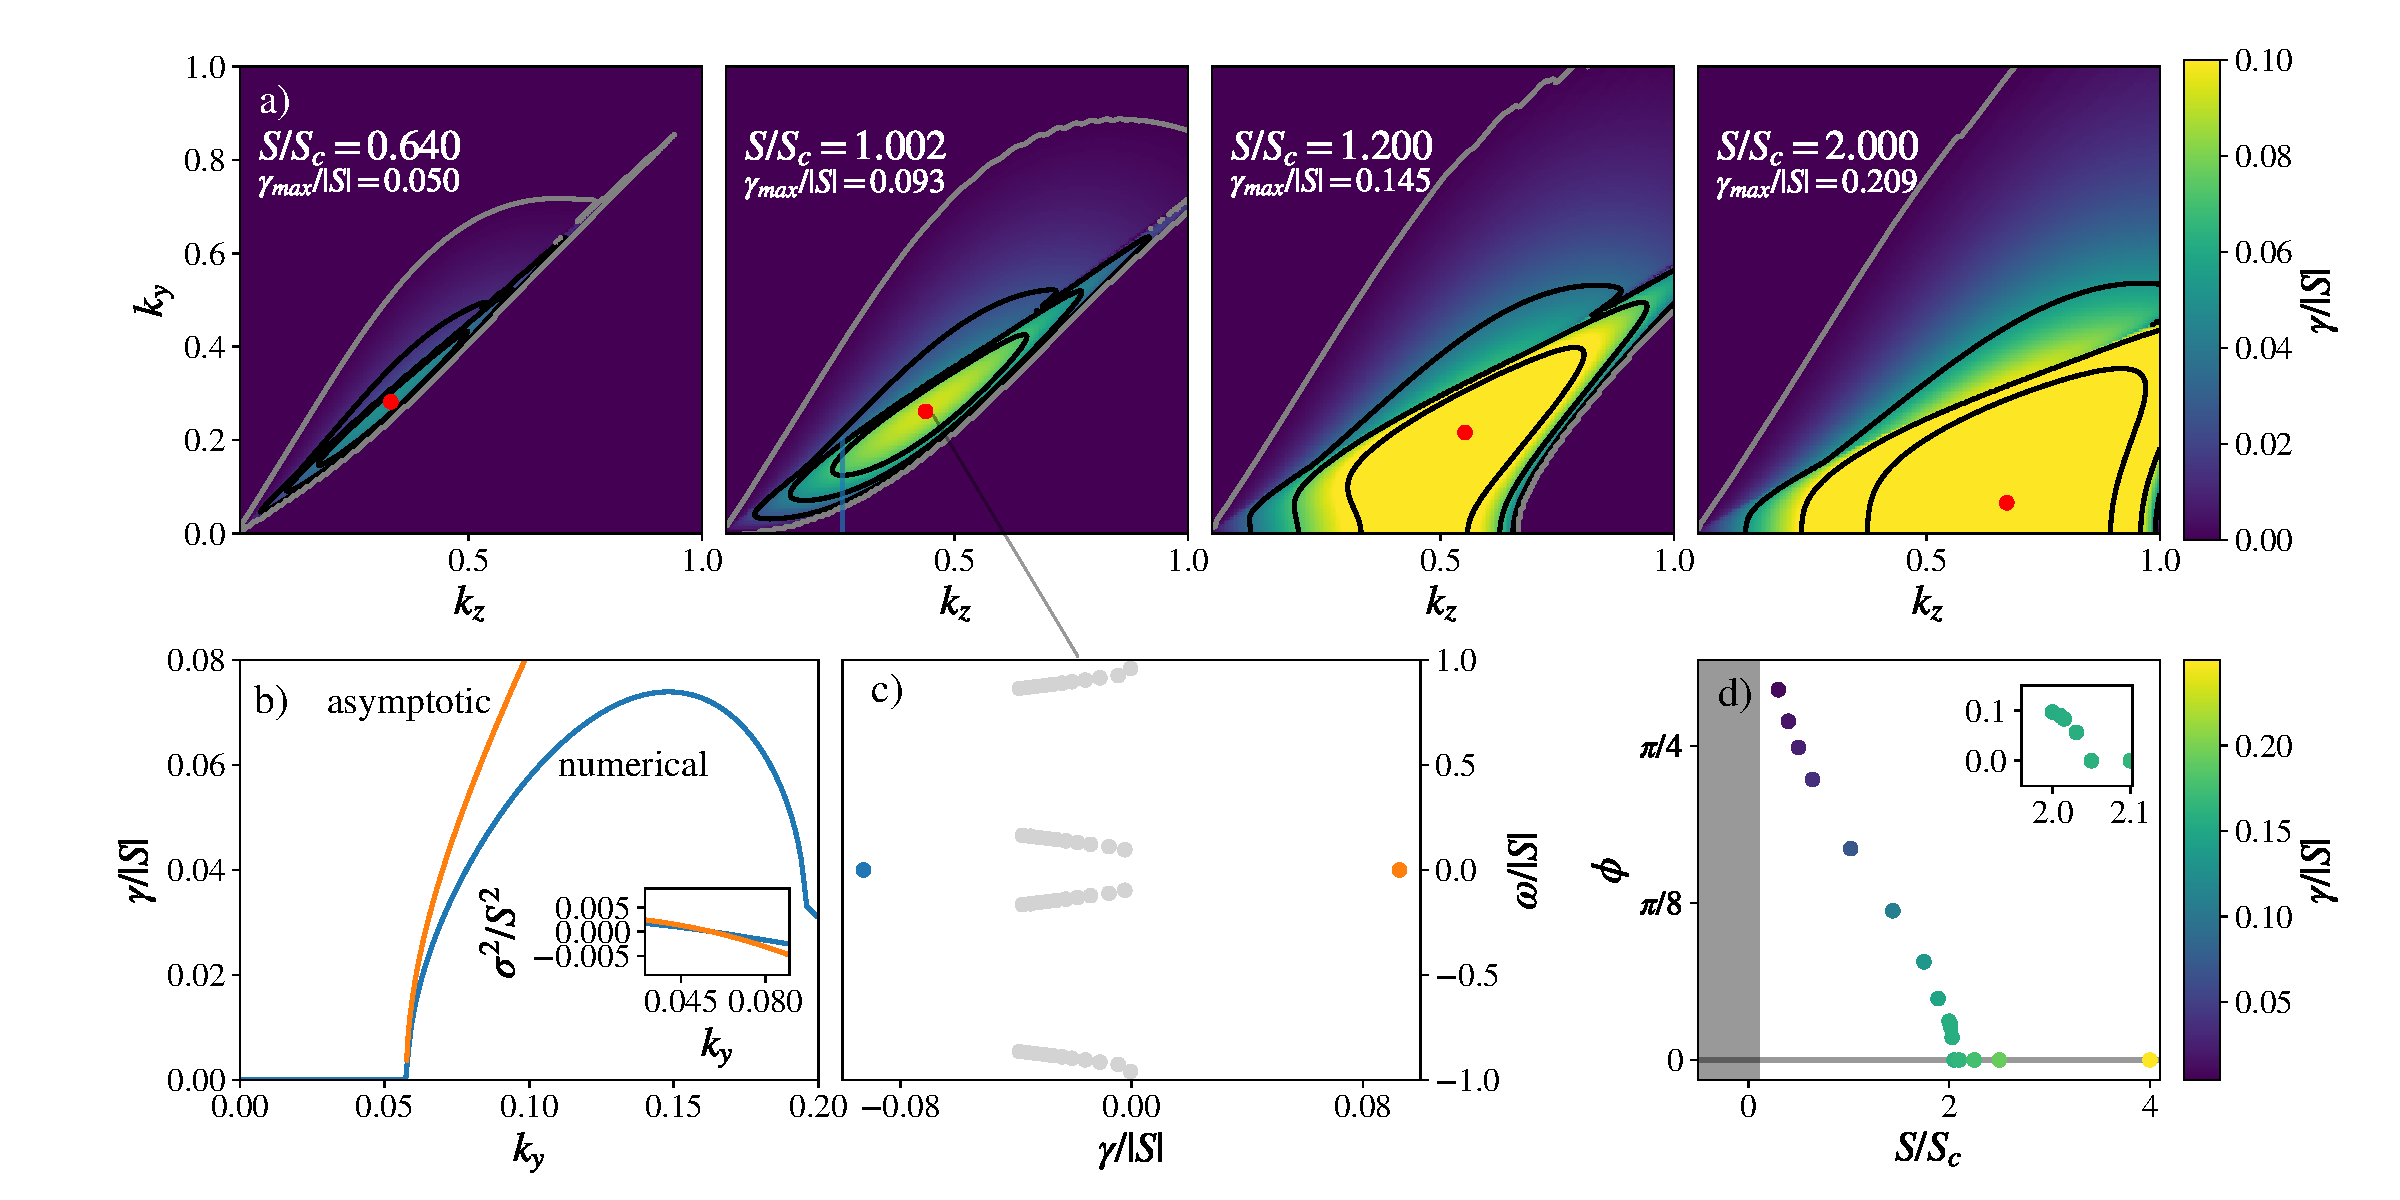
\includegraphics[width=\textwidth]{fig_1.pdf}
  \caption{Growth rates for three-dimensional MRI modes. 
  a) growth rates $\gamma$ over a grid of $k_{y}$ and $k_{z}$ for four values of supercriticality $\SSC$. 
  The five black contours are equally spaced between zero and the maximum growth rate.
  The gray contour highlights $\gamma=0$; the red dots indicate the fastest growing mode. 
Two dimensional modes occur at $k_y = 0$ on the bottom of each figure.
  At $\SSC=0.640$, there are no two dimensional modes. 
  b) Growth rate vs $k_{y}$ for $k_{z}=0.259$ at $\SSC=1.002$ (highlighted by the blue line in a). 
  The orange line gives the asymptotic result from equation~(\ref{eq:asymp}) and the blue line are the numerical results. 
  The asymptotic form is valid as $\SSC\to1$ and $k_{y}\ll1$.) c) The full discrete spectrum of the MRI for $(k_{y},k_{z})\simeq(0.263,0.447)$. 
  The unstable mode is plotted in orange, its stable complex conjugate is blue, and all other modes are gray. 
  d) The phase angle, $\arctan(k_{y}/k_{z})$, as a function of $\SSC$ showing the exact transition to purely two-dimensional fastest modes ($\phi=0$) at $\SSC\gtrsim2.05$. }
  \label{fig:growth_rate}
\end{figure*}

Our two main results are: 
(I) When the first two-dimensional mode becomes unstable, there already exist three-dimensional modes with positive growth rate. 
(II) At sufficiently large criticality, the fastest-growing mode becomes purely two-dimensional. 
These results are pertinent in two ways. 
First, the MRI contains a substantial ``Goldilocks regime" with possible direct dynamo action, and this regime likely applies to stellar interiors and laboratory experiments. 
Second, our results accord with well-established results for accretion disks that expect two-dimensional primary modes.
Figure~\ref{fig:growth_rate}a shows the growth rates for four values of $\SSC$. 
At $\SSC=1.02$, the maximum growth rate ($\gamma_{\max}/|S|=0.093$) happens at $(k_{y},k_{z})\simeq(0.263,0.447)$.
Two-dimensional instability occurs for modes with finite growth rates at $k_y = 0$ along the bottom of the figure.
In all cases in figure~\ref{fig:growth_rate}a, the maximum growth rate does not occur along this line, indicating the dominance of three-dimensional modes.
The first panel of figure~\ref{fig:growth_rate}a shows $\SSC=0.640$, which contains only three-dimensional instability: the zero growth rate contour (highlighted in grey) does not intercept the $x$-axis.

The MRI's preference for three-dimensional modes can be predicted analytically.
We analyze equations~(\ref{eq:mhd}-\ref{eq:divu}) asymptotically close to $S_{c}$, and compute the leading-order correction to the growth rate from three-dimensional effects assuming $\SSC=1+\epsilon^{2}R$, $k_{z}\sim\mathcal{O}(\epsilon)$, $\sigma\sim{k_{y}}\sim\mathcal{O}(\epsilon^{2})$, 
\begin{equation}\label{eq:asymp}
\sigma^{2}=\frac{q\,B_{0}^{2}}{(q+1)}\left[ k_{z}^{2}\left(R-\frac{d^2}{\pi^{2}}k_{z}^{2}\right)+\Upsilon\,k_{y}^{2}\right]+\ldots,
\end{equation}
where
\begin{equation}
\Upsilon=\frac{\left(\pi^{2}+6\right) q+\pi^{2}-6}{12}\approx1.31\quad\text{for}\quad{q}=\frac{3}{4}.
\end{equation}
The first term in equation~(\ref{eq:asymp}) results from the two-dimensional calculation.
The second term is positive definite: it \emph{always} leads to enhanced growth rates when $k_{y}\neq0$ and ultraviolet divergence in the absence of higher-order effects.

Figure~\ref{fig:growth_rate}b compares the numerical growth rates for $\SSC=1.002$ between $0\le{k_{y}}\le0.2$ to the asymptotic approximation, showing good agreement where the latter is valid.
Figure~\ref{fig:growth_rate}c shows the full spectrum for $\SSC=1.02$.
The plot shows a purely growing/decaying complex-conjugate pair (orange/blue dots on the real axis) consistent with equation~(\ref{eq:asymp}).
The other stable modes (gray dots) are rotationally modified Alfv\'{e}n waves found in left- and right-going pairs, consistent with the analytic predictions for two-dimensional stability calculations.
We reject spurious eigenvalues by using \texttt{eigentools} \footnote{\protect\url{https://bitbucket.org/jsoishi/eigentools}} to solve equations~(\ref{eq:mhd}-\ref{eq:divu}) at two resolutions and retain only pairs equal to within one part in $10^{-6}$.

\begin{figure}[h!]
  \centering
  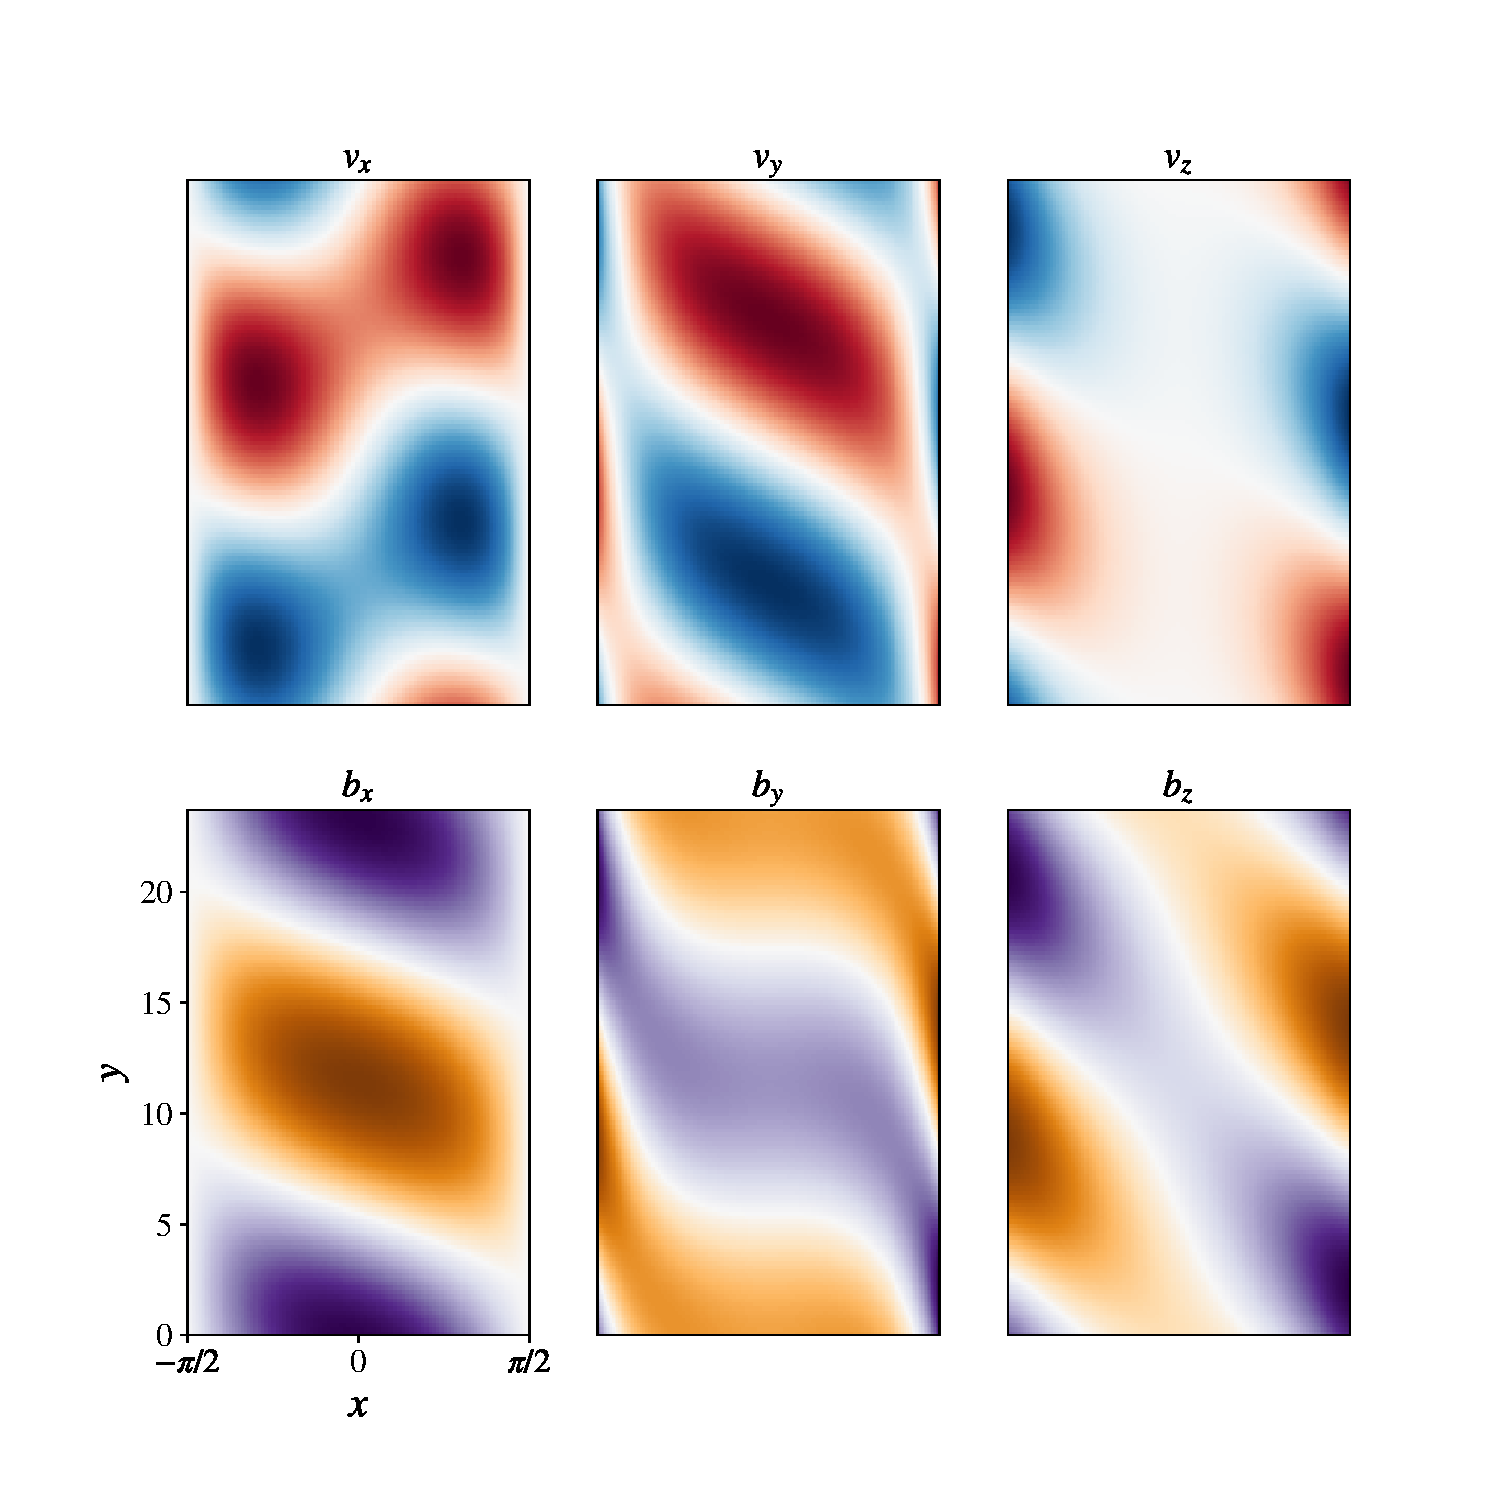
\includegraphics[width=\columnwidth]{eigvecs_xy_run_11_ideal_single_mode.pdf}
  \caption{\textit{Ideal} eigenvectors of the velocity and magnetic field perturbations for the most unstable mode when $\SSC=1.02$, and $\eta=\nu=0$; calculations at $\eta=\nu=10^{-5}$ are indistinguishable.
  The top row shows $v_{x}$, $v_{y}$, $v_{z}$ (red is negative, blue positive); the bottom row shows $b_{x}$, $b_{y}$, $b_{z}$ (purple is negative, orange positive). 
The amplitudes are arbitrary because of linearity.}
  \label{fig:eigvec}
\end{figure}

Numerical simulations of the MRI in accretion disks consistently show axisymmetric modes dominating the early evolution of the MRI before breaking down into 3D MHD turbulence \citep{1995ApJ...440..742H,2018ApJ...853..174H,2019ApJS..241...26D}. 
These ``channel modes'' are exact non-linear solutions for $x$-shearing-periodic domains, and can only saturate via parasitic shear instabilities \citep{1994ApJ...432..213G}.
Impenetrable and stress-free boundary conditions are more applicable to stellar interiors. 
But even in disks, any kind of finite radial extent will cutoff the unbounded growth of channel modes. 
We reconcile our results with earlier simulations by showing that the MRI indeed prefers two dimensions for the larger values of criticality found in disk simulations. 
Figure~\ref{fig:growth_rate}d shows the phase angle $\phi=\arctan(k_{y}/k_{z})$ of the fastest growing mode as function of $\SSC$.
The overall critical shear for three-dimensional modes is $S_{c,\text{3D}}\simeq0.102S_c$.
Above $\SSC\gtrsim2.05$, $\phi$ becomes zero, indicating that axisymmetric modes have the fastest growth rates.
For the fiducial run in \citet{1996ApJ...464..690H}, $\SSC\simeq4.84$ (most works use similar values).
Thus, our theory predicts axisymmetric modes should dominate the linear dynamics for parameters studied in prior numerical simulations.

\begin{figure}[h!]
  \includegraphics[width=\columnwidth]{{mean_field_alpha_run_11_output.h5}.pdf}
  \caption{Velocity-magnetic field correlations relevant to the mean electromotive force for the eigenvectors of the fastest growing mode at $\SSC = 1.02$.}
  \label{fig:correlation}
\end{figure}

Even for $\SSC> 2.05$ there are significant swaths of unstable three-dimensional modes with growth rates comparable to the maximum (figure~\ref{fig:growth_rate}a).
Also, non-normality generically accompanies non-axisymmetry in shearing systems \citep[see][]{1992MNRAS.255P..25K}.
In non-normal systems, transient amplification can occur for stable modes, and can even cause turbulence.
Therefore significant three dimensionality likely implies important non-normal behavior near onset.

Figure~\ref{fig:eigvec} shows the eigenvectors for the most unstable mode at $\SSC=1.02$ using ideal MHD. 
No critical layers can form for $\gamma\ne0$.
We therefore solve equations~(\ref{eq:mhd}--\ref{eq:divu}) without dissipation as a 2nd-order system in $\partial_{x}$ and impose $v_{x}=0$ at $x=\pm{d/2}$.
The eigenfunctions are indistinguishable from those at finite dissipation, lending additional confidence to our other results.
The tilted structures of $v_{x}$ and $v_{y}$ as well as $b_{x}$ and $b_{y}$, imply non-trivial Reynolds and Maxwell stresses.

We should expect the generation of a mean electromotive force (EMF) in the linear regime, \textit{i.e}
$\left<\boldsymbol{v}\times\boldsymbol{b}\right>\sim\,\alpha\!\left<\boldsymbol{B}_{0}\right>$.
This is significant because of the possibility of direct laminar dynamo action in regions of weak shear at large Reynolds number.
Figure~\ref{fig:correlation} shows the correlation (averaged over $y,\,z$) as a function of $x$ over the domain for $\SSC = 1.02$,
\begin{equation}
\text{EMF}\propto\frac{\left<\boldsymbol{\hat{z}}\cdot(\boldsymbol{v}\times\boldsymbol{b})\right>_{\!y,z}}{\boldsymbol{v}_{\text{rms}}\boldsymbol{b}_{\text{rms}}},
\end{equation}
where ``rms'' is denotes the average over the whole domain. 
The correlation is independent of the arbitrary normalisation of the linear eigenvectors.
The non-zero correlation shows the tendency for back reaction on the mean magnetic field.

MRI dynamos have been studied in a number of different contexts \citep{2007PhRvL..98y4502R,2011ApJ...740...18O,2015PhRvL.114h5002S}, but all except one focused on turbulent dynamos. 
The lone exception, \citet{2016MNRAS.462..818B}, numerically found the exponential growth of mean magnetic fields during the linear growth phase of the MRI far from stability.
Our work explains this result in terms of purely linear dynamics:
non-axisymmetric MRI unstable modes drive the dynamo growth of magnetic fields.


\begin{figure}[h!]
  \centering
  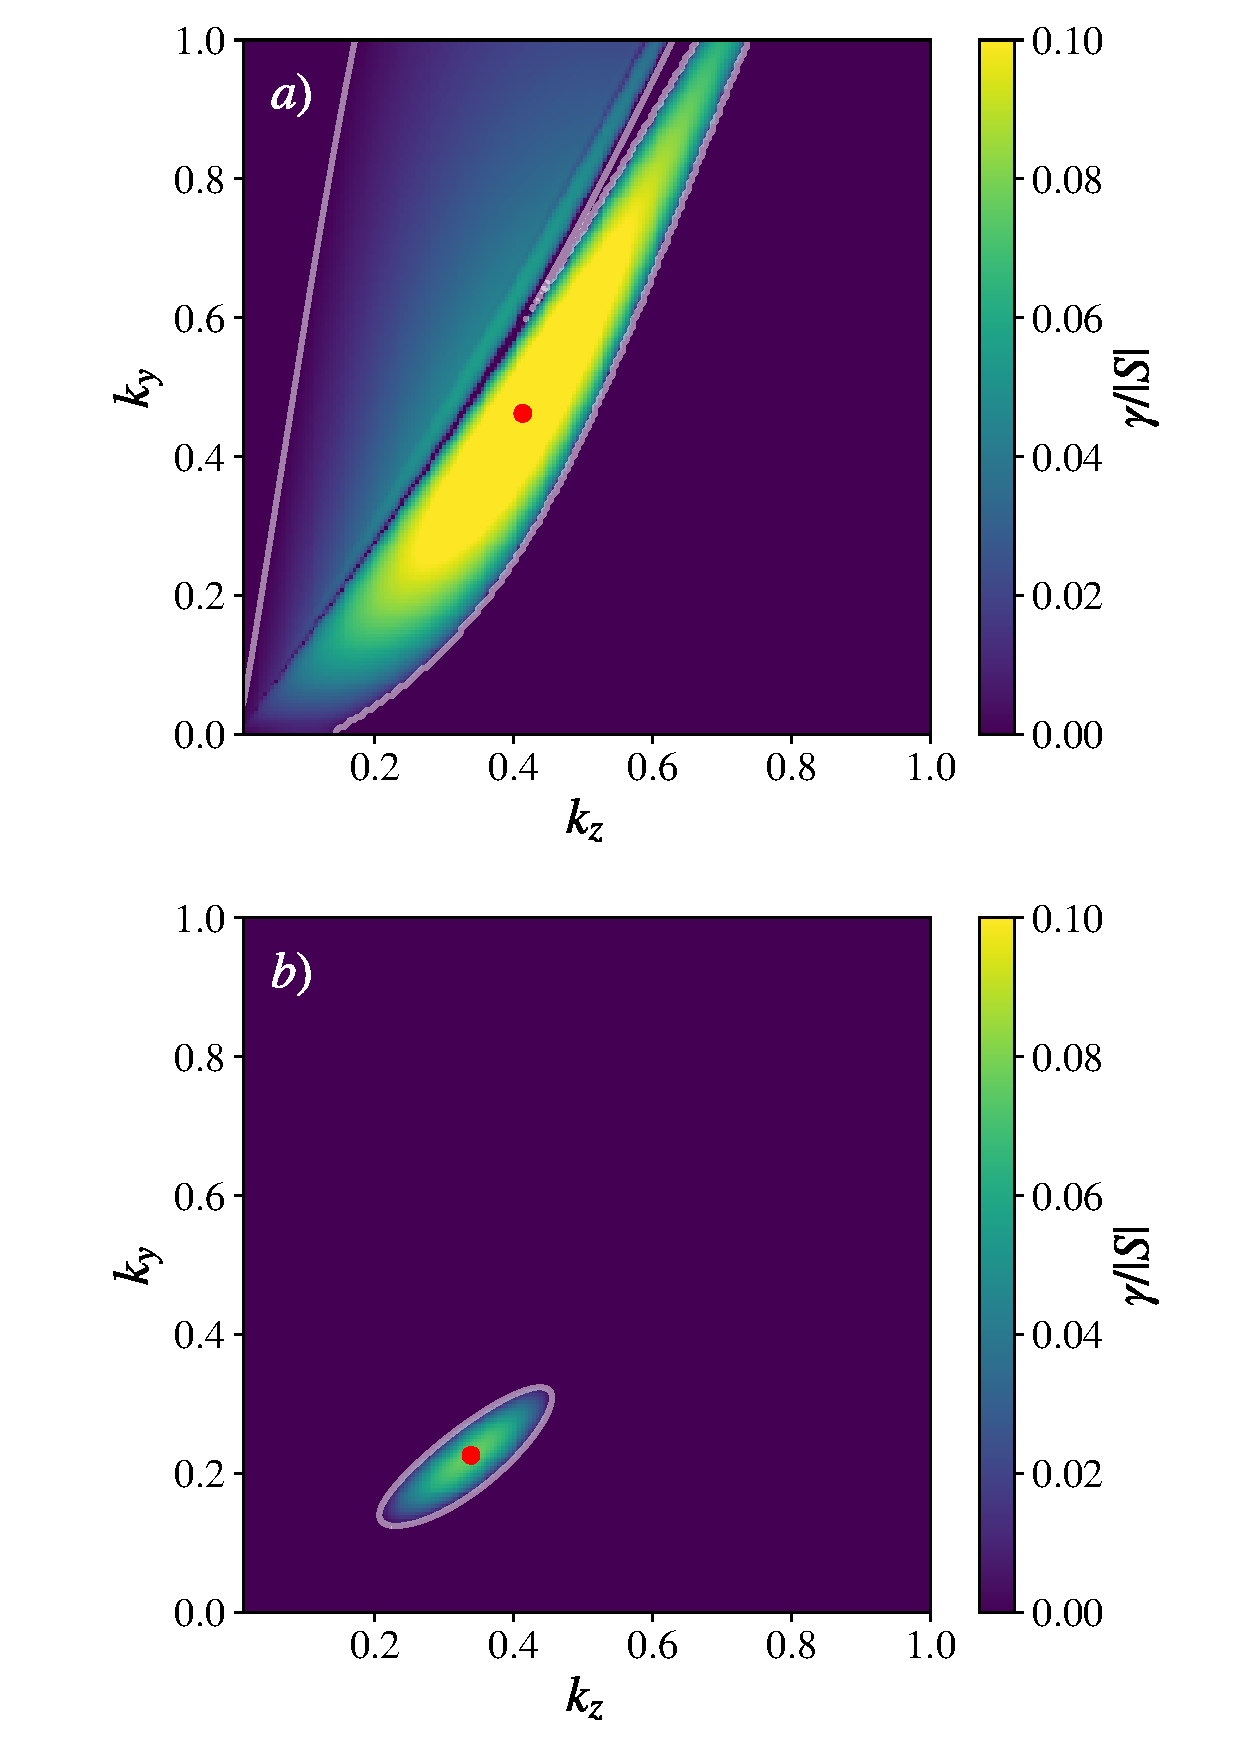
\includegraphics[width=\columnwidth]{low_rossby_liquid_metal_growth_rates.pdf}
  \caption{(a) Growth rates for $q=1/10$ relevant to the stellar interiors. 
  (b) Growth rates for MRI near onset at liquid metal-like diffusivities, $\nu=10^{-6}$, $\eta=0.1$.
The lack of two dimensional instability is evident by the fact that the zero contour does not intercept the x-axis.}
  \label{fig:other_params}
\end{figure}
Finally, we vary two important parameters:
$q$ and the magnetic Prandtl number $\Prm=\nu/\eta$.
Figure~\ref{fig:other_params} shows the growth rates for $\SSC=1.02$.
The upper panel shows $q=1/10$ (addressing a possible range within stellar interiors) holding all other parameters equal to their fiducial values.
The growth rates show similar behavior to the $q=3/4$ cases, \textit{i.e.}, dominated by three-dimensional modes with $\gamma_{\max}/|S|\simeq0.1$.
The lower panel shows $\nu=10^{-6}$ and $\eta=0.1$ with all other parameters equal to their fiducial values. 
This case is relevant to liquid metals e.g., the Princeton MRI experiment \citep{2002JFM...462..365G}
at $\Prm=10^{-5}$. 
Our results are for the rotating plane Couette geometry (Taylor-Couette in the small-gap limit $R_{2}\approx{R}_{1}$) with highly idealized boundary conditions.
It is nevertheless quite interesting that, near onset, the low-$\Prm$ MRI is \emph{only} unstable to three-dimensional modes.

Our results show that three-dimensional modes grow faster than two-dimensional modes whenever the MRI is near its critical shear values.
While we mainly focus on the ideal Keplerian case ($q=3/4$), we also demonstrate robustness for low Rossby ($q=1/10$) and Prandtl numbers ($\Prm=10^{-5}$).
There are several important future directions this work suggests.
First, the Sun possesses two internal shear layers with inwardly increasing shear, the high-latitude tachocline, and the near-surface shear layer (NSSL). 
Past work has already pointed out the possibility of the small-scale MRI in the Sun using local analysis \citep{2007ApJ...667L.207P,2011MNRAS.411L..26M,2014ApJ...787...21K}.
The NSSL, in particular, may also host slower MRI-driven dynamics; despite containing small-scale convection.
It is therefore crucial to further elucidate the nonlinear saturation of the 3D MRI, along with its robustness to convection.
Second, our low-$\Prm$ results suggest that three-dimensional MRI modes may be the easiest to excite in liquid metal experiments.
Determining possible non-axisymmetric signatures in Taylor-Couette experiments requires followup work using more realistic boundary conditions and geometry. 
Our prior work on the axisymmetric MRI \citep{2017ApJ...841....1C,2017ApJ...841....2C} shows only small differences between rotating plane and cylindrical Taylor-Couette geometries. 
We fully expect the general three-dimensional features of the MRI to persist in more complex applications. 


\begin{acknowledgments}
We thank Steve Tobias for helpful conversations on this work.
Oishi, Baxter, and Brown acknowledge support from NASA LWS grant No. NNX16AC92G.
Oishi also acknowledges support from Research Corporation Scialog Collaborative Award (TDA) ID\#24231. 
Computations were performed on the \emph{Leavitt} cluster at the Bates College High Performance Computing Center.

\end{acknowledgments}

\bibliography{mri}

\end{document}


%  LocalWords:  Magnetorotational Oishi Lewiston Vasil NSW Lecoanet
%  LocalWords:  magnetorotational Keplerian magnetofluid Prandtl MHD
%  LocalWords:  dimensionality Couette axisymmetric linearized RSPSA
%  LocalWords:  magnetohydrodynamic Navier Dt Dj dV dx Alfv Rossby fd
%  LocalWords:  hydrodynamical ODEs Dedalus arXiv supercriticality nd
%  LocalWords:  criticality eigenvectors fiducial axisymmetry NSSL
%  LocalWords:  eigenfunctions eigenmodes diffusivities tachocline
%  LocalWords:  Tobias JSO LWS NNX Scialog TDA Leavitt mri
